\setcounter{chapter}{0}
\chapter{Rotational Motion}

\section{Rotational Motion under Constant Angular Acceleration}

\begin{itemize}
	\item The object rotates around an axis in \textbf{rotational motion}.
	\item The axis of rotation can change.
	\item The Earth, for example, rotates on its own axis.

	\item Circular motion is a type of a two dimensional motion, along \textbf{the circumference of a circle}.
	\item The distance between the center of mass and the axis of rotation remains \textbf{fixed}.
	\item Artificial satellites, for example, orbit the Earth at a fixed altitude.

\begin{figure}[htbp]
  \centering
  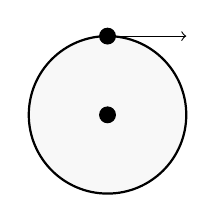
\begin{tikzpicture}[scale=1]
    \draw[thick, fill=gray!10, fill opacity=0.5] (0,0) circle (1);
    \filldraw (0,0) circle (0.1);
    \filldraw (0,1) circle (0.1);
    \draw[->] (0,1) -- (1,);
  \end{tikzpicture}%
  \hfil
  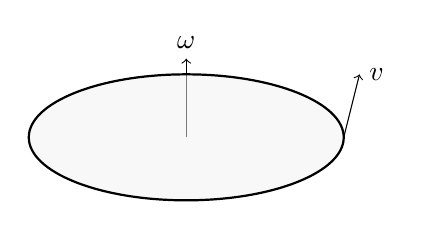
\begin{tikzpicture}[z={(0cm,1cm)}]
    %Axis
    \draw[->] (0,0,0) -- (0,0,1) node[above] {$\omega$};

    %Circle
    \draw[thick, fill=gray!10, fill opacity=0.5] (0,0) ellipse (2cm and 0.8cm);
    \draw[->] (2cm,0) -- (2.2cm,0.8cm) node[right] {$v$};
  \end{tikzpicture}
  \caption{Rotational motion \& Circular motion}
\end{figure}

	\item \textbf{Rigid body:} size \& shape do not change as it moves;
	\item \textbf{Rigid body} in \textbf{rotational motion:} all the particles undergo \textbf{circular motion}
	\item \textbf{Rigid body} in \textbf{rotation:} its angular velocity changes therefore undergoes \textbf{angular acceleration}
\end{itemize}


$\boldsymbol{\alpha}$ is \textbf{negative} when rigid body is rotating:
\begin{itemize}
	\item \textbf{anti-clockwise \& slowing down}
	\item \textbf{clockwise \& speeding up}
\end{itemize}

$\boldsymbol{\alpha}$ is \textbf{positive} when rigid body is rotating:
\begin{itemize}
	\item \textbf{anti-clockwise \& speeding up}
	\item \textbf{clockwise \& slowing down}
\end{itemize}

If angular velocity changes at a constant rate:
angular acceleration is constant and
the rotational motion is under \textbf{constant angular acceleration}

\begin{align}
	\alpha &= \frac{\omega - \omega_0}{\tau} \nonumber \\
	\omega &= \omega_0 + \alpha\tau \\
	\text{Average angular speed: } \bar{\omega} &=  \frac{\omega + \omega_0}{2} \\
	\theta &= \bar{\omega}\tau \nonumber \\
	\theta &= \omega_0\tau + \frac12 \alpha\tau^2 \\
	\omega^2 &= \omega_0\tau + 2 \alpha \theta
\end{align}

Units:
\begin{align*}
	\text{angular displacement: } & \text{radian } (rad) = 2\pi \\
	\text{angular velocity: } & \text{radian per second } (rad/s) \\
	\text{angular acceleration: } & \text{radian per second squared } (rad/s^2)
\end{align*}

\section{Relation Between Angular \& Linear Quantities}
All particles of the body move in a circle perpendicular to the axis

The direction of linear velocity is tangent to the path called \textbf{tangential velocity}

When linear velocity change, the object have \textbf{tangential acceleration}

$ a_r = r\alpha $

\textbf{The right-hand rule} \\
\begin{itemize}
	\item \textbf{The fingers}: direction of rotation
	\item \textbf{The thumb}: direction of angular velocity vector
\end{itemize}

The angular velocity is:
\begin{itemize}
	\item \textbf{increasing:} angular acceleration vector points in the \textbf{same} direction
	\item \textbf{decreasing:} angular acceleration vector points in the \textbf{opposite} direction
\end{itemize}

\section{Centripetal Acceleration}
\begin{itemize}
	\item Constant speed $v$: \textbf{uniform circular motion}
	\item The magnitude of the velocity remains constant but the direction of velocity continuously changes
	\item Continuously accelerated even when speed is constant $ (v_1 = v_2 = v) $
	\item $\Delta t$ approaches zero: \textbf{instantaneous acceleration}
	\item $\Delta t$ is very small: $\Delta s$ \& $\Delta \theta$ are also very small
		and $\vec{v_2} \parallel \vec{v_1}$ 
	\item $\Delta\vec{v}$ perpendicular to both of them
		and points toward the center of the circle
	\item Acceleration $\vec{a}$ is in the same direction as $\Delta\vec{v}$,
		and is \textbf{centripetal acceleration}
	\item The centripetal (radial) acceleration can be determined as follow:

\end{itemize}

Therefore, 
\begin{align}
	a_c &= \frac{v^2}{r} \\
	v &= r\omega \\
	a_c &= r\omega^2
\end{align}

For \textbf{uniform circular motion},
centripetal acceleration vector points towards the center
while the linear velocity vector is tangential

Centripetal acceleration \& linear velocity are perpendicular to each other

For \textbf{non-uniform circular motion},
angular speed is changing and the object experiences the angular acceleration

There is tangential acceleration in addition to centripetal acceleration

\begin{align}
	\vec{a} &= \vec{a_c} + \vec{a_r}
\end{align}

Unlike tangential acceleration,
centripetal acceleration is present in both uniform \& non-uniform circular motion.

\begin{align}
	a &= \sqrt{a_c^2 + a_r^2} \\
	tan \phi &= \frac{a_r}{a_c}
\end{align}


\section{Forces in Circular Motion}
2 basic forces:
\begin{itemize}
	\item \textbf{Centripetal force:} towards the centre of the circular path
	\item \textbf{Centrifugal force:} away from the centre
\end{itemize}

Newton's third law: the ball exerts a reaction force on the hand

When the car is moving with constant velocity along a straight road:
there is no net force on the person

When the car moves around a curve:
the person feels a \textbf{outward force}---centrifugal force---exerted on him

Centrifugal force is
caused by the effect of inertia and is not a real force
an apparent or fictitious force: equal \& opposite to the centripetal force
